\documentclass[a4paper, 11pt]{article}
% Some Computer Society conferences also require the compsoc mode option,
% but others use the standard conference format.
%
% If IEEEtran.cls has not been installed into the LaTeX system files,
% manually specify the path to it like:
% \documentclass[conference]{../sty/IEEEtran}





% Some very useful LaTeX packages include:
% (uncomment the ones you want to load)


% *** MISC UTILITY PACKAGES ***
%
%\usepackage{ifpdf}
% Heiko Oberdiek's ifpdf.sty is very useful if you need conditional
% compilation based on whether the output is pdf or dvi.
% usage:
% \ifpdf
%   % pdf code
% \else
%   % dvi code
% \fi
% The latest version of ifpdf.sty can be obtained from:
% http://www.ctan.org/pkg/ifpdf
% Also, note that IEEEtran.cls V1.7 and later provides a builtin
% \ifCLASSINFOpdf conditional that works the same way.
% When switching from latex to pdflatex and vice-versa, the compiler may
% have to be run twice to clear warning/error messages.


%- algemene verloop doorheen dag/week
%- recurring patterns tussen dagen
%- drukkere/rustigere channels
%- 2.4 vs 5 (gelijkaardig aan het vorige)



% *** CITATION PACKAGES ***
%
\usepackage{cite}
% cite.sty was written by Donald Arseneau
% V1.6 and later of IEEEtran pre-defines the format of the cite.sty package
% \cite{} output to follow that of the IEEE. Loading the cite package will
% result in citation numbers being automatically sorted and properly
% "compressed/ranged". e.g., [1], [9], [2], [7], [5], [6] without using
% cite.sty will become [1], [2], [5]--[7], [9] using cite.sty. cite.sty's
% \cite will automatically add leading space, if needed. Use cite.sty's
% noadjust option (cite.sty V3.8 and later) if you want to turn this off
% such as if a citation ever needs to be enclosed in parenthesis.
% cite.sty is already installed on most LaTeX systems. Be sure and use
% version 5.0 (2009-03-20) and later if using hyperref.sty.
% The latest version can be obtained at:
% http://www.ctan.org/pkg/cite
% The documentation is contained in the cite.sty file itself.
\usepackage{siunitx}
\usepackage[pdftex]{graphicx}
  % declare the path(s) where your graphic files are
\graphicspath{{../images/}}


\usepackage{hyperref}


% *** MATH PACKAGES ***
%
\usepackage{amsmath}
% A popular package from the American Mathematical Society that provides
% many useful and powerful commands for dealing with mathematics.
%
% Note that the amsmath package sets \interdisplaylinepenalty to 10000
% thus preventing page breaks from occurring within multiline equations. Use:
%\interdisplaylinepenalty=2500
% after loading amsmath to restore such page breaks as IEEEtran.cls normally
% does. amsmath.sty is already installed on most LaTeX systems. The latest
% version and documentation can be obtained at:
% http://www.ctan.org/pkg/amsmath





% *** SPECIALIZED LIST PACKAGES ***
%
%\usepackage{algorithmic}
% algorithmic.sty was written by Peter Williams and Rogerio Brito.
% This package provides an algorithmic environment fo describing algorithms.
% You can use the algorithmic environment in-text or within a figure
% environment to provide for a floating algorithm. Do NOT use the algorithm
% floating environment provided by algorithm.sty (by the same authors) or
% algorithm2e.sty (by Christophe Fiorio) as the IEEE does not use dedicated
% algorithm float types and packages that provide these will not provide
% correct IEEE style captions. The latest version and documentation of
% algorithmic.sty can be obtained at:
% http://www.ctan.org/pkg/algorithms
% Also of interest may be the (relatively newer and more customizable)
% algorithmicx.sty package by Szasz Janos:
% http://www.ctan.org/pkg/algorithmicx


\usepackage[font=small]{caption}
\makeatletter
\renewcommand{\fnum@figure}{Fig. \thefigure}
\makeatother
\usepackage{wrapfig}

% *** ALIGNMENT PACKAGES ***
%
%\usepackage{array}
% Frank Mittelbach's and David Carlisle's array.sty patches and improves
% the standard LaTeX2e array and tabular environments to provide better
% appearance and additional user controls. As the default LaTeX2e table
% generation code is lacking to the point of almost being broken with
% respect to the quality of the end results, all users are strongly
% advised to use an enhanced (at the very least that provided by array.sty)
% set of table tools. array.sty is already installed on most systems. The
% latest version and documentation can be obtained at:
% http://www.ctan.org/pkg/array


% IEEEtran contains the IEEEeqnarray family of commands that can be used to
% generate multiline equations as well as matrices, tables, etc., of high
% quality.




% *** SUBFIGURE PACKAGES ***
%\ifCLASSOPTIONcompsoc
%  \usepackage[caption=false,font=normalsize,labelfont=sf,textfont=sf]{subfig}
%\else
%  \usepackage[caption=false,font=footnotesize]{subfig}
%\fi
% subfig.sty, written by Steven Douglas Cochran, is the modern replacement
% for subfigure.sty, the latter of which is no longer maintained and is
% incompatible with some LaTeX packages including fixltx2e. However,
% subfig.sty requires and automatically loads Axel Sommerfeldt's caption.sty
% which will override IEEEtran.cls' handling of captions and this will result
% in non-IEEE style figure/table captions. To prevent this problem, be sure
% and invoke subfig.sty's "caption=false" package option (available since
% subfig.sty version 1.3, 2005/06/28) as this is will preserve IEEEtran.cls
% handling of captions.
% Note that the Computer Society format requires a larger sans serif font
% than the serif footnote size font used in traditional IEEE formatting
% and thus the need to invoke different subfig.sty package options depending
% on whether compsoc mode has been enabled.
%
% The latest version and documentation of subfig.sty can be obtained at:
% http://www.ctan.org/pkg/subfig




% *** FLOAT PACKAGES ***
%
%\usepackage{fixltx2e}
% fixltx2e, the successor to the earlier fix2col.sty, was written by
% Frank Mittelbach and David Carlisle. This package corrects a few problems
% in the LaTeX2e kernel, the most notable of which is that in current
% LaTeX2e releases, the ordering of single and double column floats is not
% guaranteed to be preserved. Thus, an unpatched LaTeX2e can allow a
% single column figure to be placed prior to an earlier double column
% figure.
% Be aware that LaTeX2e kernels dated 2015 and later have fixltx2e.sty's
% corrections already built into the system in which case a warning will
% be issued if an attempt is made to load fixltx2e.sty as it is no longer
% needed.
% The latest version and documentation can be found at:
% http://www.ctan.org/pkg/fixltx2e


%\usepackage{stfloats}
% stfloats.sty was written by Sigitas Tolusis. This package gives LaTeX2e
% the ability to do double column floats at the bottom of the page as well
% as the top. (e.g., "\begin{figure*}[!b]" is not normally possible in
% LaTeX2e). It also provides a command:
%\fnbelowfloat
% to enable the placement of footnotes below bottom floats (the standard
% LaTeX2e kernel puts them above bottom floats). This is an invasive package
% which rewrites many portions of the LaTeX2e float routines. It may not work
% with other packages that modify the LaTeX2e float routines. The latest
% version and documentation can be obtained at:
% http://www.ctan.org/pkg/stfloats
% Do not use the stfloats baselinefloat ability as the IEEE does not allow
% \baselineskip to stretch. Authors submitting work to the IEEE should note
% that the IEEE rarely uses double column equations and that authors should try
% to avoid such use. Do not be tempted to use the cuted.sty or midfloat.sty
% packages (also by Sigitas Tolusis) as the IEEE does not format its papers in
% such ways.
% Do not attempt to use stfloats with fixltx2e as they are incompatible.
% Instead, use Morten Hogholm'a dblfloatfix which combines the features
% of both fixltx2e and stfloats:
%
% \usepackage{dblfloatfix}
% The latest version can be found at:
% http://www.ctan.org/pkg/dblfloatfix




% *** PDF, URL AND HYPERLINK PACKAGES ***
%
%\usepackage{url}
% url.sty was written by Donald Arseneau. It provides better support for
% handling and breaking URLs. url.sty is already installed on most LaTeX
% systems. The latest version and documentation can be obtained at:
% http://www.ctan.org/pkg/url
% Basically, \url{my_url_here}.




% *** Do not adjust lengths that control margins, column widths, etc. ***
% *** Do not use packages that alter fonts (such as pslatex).         ***
% There should be no need to do such things with IEEEtran.cls V1.6 and later.
% (Unless specifically asked to do so by the journal or conference you plan
% to submit to, of course. )


% correct bad hyphenation here
\hyphenation{op-tical net-works semi-conduc-tor}


\begin{document}
%
% paper title
% Titles are generally capitalized except for words such as a, an, and, as,
% at, but, by, for, in, nor, of, on, or, the, to and up, which are usually
% not capitalized unless they are the first or last word of the title.
% Linebreaks \\ can be used within to get better formatting as desired.
% Do not put math or special symbols in the title.
\title{A study on the usage of the wireless signal spectrum in a City of Things network}


% author names and affiliations
% use a multiple column layout for up to three different
% affiliations
\author{
	Jakob Struye (20120612)\\ 
    Thomas Hendriks (20139858)\\
}

How bad is it, in general? 
Are there patterns, e.g. daily recurrence? 
Advanced: how can you ensure data quality, i.e., how to validate the results? 

\maketitle

% As a general rule, do not put math, special symbols or citations
% in the abstract

\tableofcontents
\clearpage

\section{Introduction}
% no \IEEEPARstart
Most of the radio spectrum requires a license to operate on. Devices emitting Radio Frequency (RF) energy without a license often use one of the unlicensed Industrial, Scientific and Medical (ISM) radio bands. The most well-known of these bands is the 100MHz wide band centered around 2.45GHz, often called the 2.4GHz band. Many consumer devices such as wireless mice and keyboards, bluetooth headphones and Radio Controlled (RC) cars communicate in the 2.4GHz band. Furthermore most IEEE 802.11 (Wi-Fi) routers operate in the 2.4GHz band. In addition 802.11ac routers operating in the 5GHz range often use the 5GHz ISM band (which actually ranges from 5.725GHz to 5.875GHz). Some other bands in the 5GHz are also allowed for 802.11ac, although more restrictions, such as indoors-use only, apply there~\cite{50ism}. These ISM bands were originally intended and still used for devices emitting RF energy for purposes other than communication. The most common such application is the microwave oven. All this leads to high interference in these bands. In this paper, we investigate how bad this 2.4GHz and 5GHz interference actually is in the city of Antwerp. \\ \\
To measure this interference we use the City of Things (CoT) network, operated by research institute imec\footnote{\url{https://www.imec-int.com/en/home}}. This network consists of hundreds of sensors and wireless gateways positioned around the city of Antwerp. On 11 of these gateways, we sampled activity on the 2.4GHz and 5GHz bands every 2 minutes for 12 days, including a Monday-to-Sunday week. The main motivation of this experiment is to investigate whether interference around the gateways is significant enough to pose a problem for the network. Next to the general magnitude of the interference, we look for patterns in daily and weekly variation of the interference.
\section{Measuring Interference}
All used nodes have a COMPEX WLE900VX-7A network adapter, containing a Qualcomm Atheros QCA9880 wireless chipset. This 802.11ac chipset, along with all other 802.11ac and 802.11n chips by Qualcomm Atheros support a mode called \textit{spectral scan}. In this mode the chip can scan the activity on all frequencies it supports. This activity is not limited to 802.11 traffic, but is influenced by any received signal. In this mode, the chip acts as a simple spectrum analyzer. The Free and Open-Source Software (FOSS) ath9k and ath10k drivers, respectively for the 802.11n and 802.11ac Qualcomm Atheros chipsets, support this mode. Each scan is performed over a period of \SI{4}{\micro\second}. Every scanned channel is divided into 64, 128 or 256 equally wide bins. For the full channel the noise floor and Received Signal Strength Indicator (RSSI) are reported, along with a magnitude for each bin. This magnitude incidates  how the power within the channel was divided across the bins. We provide an overview of how to interpret these values in section \ref{sec:interpret}. \\
\subsection{Settings}
The ath10k version of spectral scan offers fewer options than the ath9k version. For instance the option to increase the scan time from \SI{4}{\micro\second} to \SI{2044}{\micro\second} is absent in ath10k. The only missing option relevant to our case is the \textit{chanscan} mode of spectral scan. When this mode is triggered the driver gathers a configurable number of samples for every channel it supports. We emulate this behaviour using the \textit{background} mode, which continuously scans the chipset's currently configured channel as long as it is not sending or receiving. We combine this with an \textit{iw scan} command, which listens for access point beacons for a provided list of frequencies. When providing \textit{iw scan} with a list of all supported frequencies, this closely emulates the \textit{chanscan} behaviour.
\subsection{Interpreting spectral scans} \label{sec:interpret}
Before going into the interpretation of this specific data, we provide a quick overview of the dBm unit, often used to express power ratios. The regular decibel (dB) unit is a dimensionless unit. In contrast dBm expresses absolute power in reference to watt. 0 dBm is defined as 1 milliwatt (mW). For each increase of 3dBm, the power in mW doubles, and for each increase of 10dBm, the power is multiplied by 10. Milliwatt-to-dBm conversion is calculated using the formula\\ \\ $dBm = 10 log_{10}(\dfrac{x}{\SI{1}{\milli\watt}})$, with $x$ the power in mW.\\ \\ A negative dBm power simply means the power is less than \SI{1}{\milli\watt}. By using dBm, very small or large power values are often avoided. As power attenuates quadratically with distance, useful power values can vary dramatically.\\\\
For each channel scan, the driver reports the noise floor and RSSI value. The noise floor value is a hard-coded estimation for every channel and ranges between -94dBm and -108dBm. This value is the expected power of all noise in a channel combined. This includes noise sources such as thermal noise and cosmic noise. The chipset can only receive a singal whose power exceeds this noise floor. The RSSI value is a (unitless) integer indicating, as the name implies, the received power in the channel. While the existence of this value is part of the 802.11 specification, its calculation is not. As a result every manufacturer calculates the RSSI differently. Atheros chips follow a rather simple formula: subtracting the noise floor from the current signal strength in dBm results in the RSSI. These two values are enough to estimate the signal strength in a channel: a noise floor of -96dBm and an RSSI of 40 indicate a received signal of -56dBm.~\cite{rssi-calc}. The RSSI reported by Atheros is often limited to 60. As RSSI was originally intended to estimate signal quality within the driver, values above 60 were not interesting; -36dBm (assuming a noise floor of -96dBm) already indicates excellent reception. It appears however that in this spectral scan mode, the hardware does return RSSI values of over 60. \\
The per-bin magnitudes indicate how power is divided within the channel. To understand these values, some background about radio signaling is needed. Signals in radio communication are usually created using a technique called \textit{IQ modulation}. With this technique, the final signal is a combination of two separate signals (the in-phase or \textit{I} and the quadrature or \textit{Q} signals) whose phases are exactly 90 degrees apart. By changing only the amplitude of the \textit{I} and \textit{Q} signals, the resulting signal's amplitude and phase can attain any value. The reported bin magnitude $b(i)$ for bin $i$ is the sum of the absolute values of the \textit{I} and \textit{Q} signals' magnitudes. This magnitude in turn is the amplitude squared. The per-bin power scales quadratically with this magnitude value: if bin $i$ has twice the magnitude of bin $j$, bin $i$'s share of the channel's power is four times as large as bin $j$'s. We can compute a coefficient $c(i)$ for every bin $i \in [1,n]$ as follows:\\\\\hspace*{1.5em}$c(i) = \dfrac{b(i)^2}{\sum\limits_{j=1}^{n}b(j)^2}$ (Note that every $c(i) \in [0,1]$ and $\sum\limits_{c=1}^{n}{c(i)} = 1$.) \\\\
As the dBm power values computed from the noise floor and RSSI are not linear but rather logarithmic, we cannot simply multiply by $c(i)$ to get each bin's power value. Instead we first convert $c(i)$ to a logarithmic value: \\ \\ $c_{log}(i) = 10 log_{10}(c(i))$. \\ \\ As $log(a*b) = log(a) + log(b)$, we add this coefficient to the total logarithmic power to calculate each share's power:\\ \\ $nf + RSSI + c_{log}(i)$.\\ \\ Noting that $log(a/b) = log(a) - log(b)$, writing the formula using only the parameters returned by the spectral scan results in\\ \\ $nf + RSSI  + 10 log_{10}(b(i)^2) - 10 log_{10}(\sum\limits_{j=1}^{n}{b(j)^2})$ \\ \\
The earliest reference to this formula being used with the FOSS Atheros drivers was in an email on the ath9k-devel mailing list by Zefir Kurtisi~\cite{formula}, in reply to the Request For Comments (RFC) on spectral scan support by Simon W{\"u}nderlich. As far as we know neither this formula nor the calculation of its parameters were ever confirmed to be correct by Qualcomm Atheros. This remains an educated guess by the community.

\section{Measurements}


At first we measured the spectrum on every channel in both the 2.4GHz and the 5GHz band every 10 minutes. The visualizations of the gathered data using Simon W{\"u}nderlich's FFT\_eval tool\footnote{https://github.com/simonwunderlich/FFT\_eval} showed that a shorter time between scans would be useful. There were often large variations between two subsequent samples, showing a use for a shorter interval. Additionally we noticed some extreme outliers. Occasionally a received signal strength of 129dBm or 8GW was reported. As a steady 8GW supply would require over 35 million solar panels~\cite{gigawatt}, so this is clearly an erroneous measurement. Although this was a fairly rare phenomenon, it still occurred up to a few times in each node's almost 10 million daily samples. To avoid such erroneous samples, we remove the $n$ highest signal strength measurements from every scan. The choice of $n$ depends on the sample size. For a single-channel 2.4GHz scan, consisting of around 210 samples, we remove the top 5. We then consider the maximum signal strength among the remaining samples as the measured strength within the channel. \\
\begin{figure}[ht]
\begin{minipage}[t]{0.45\textwidth}
\centering
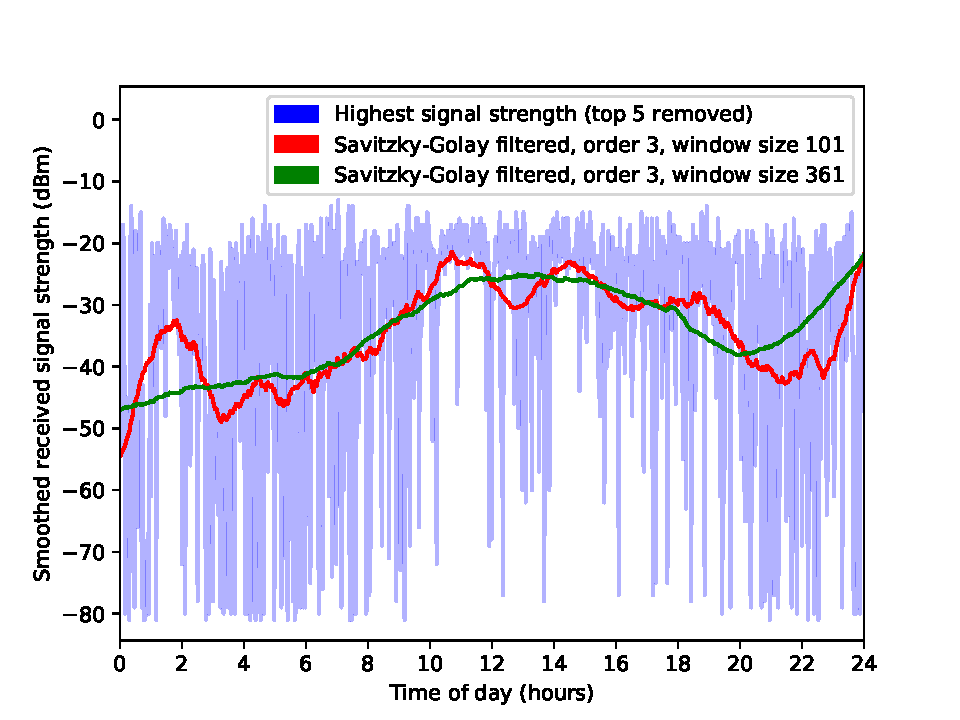
\includegraphics[width=\textwidth]{savitzky_0hours}
\caption{Savitzky-Golay smoothing.}
\label{savitzky_0}
\end{minipage}\
\begin{minipage}[t]{0.45\textwidth}
\centering
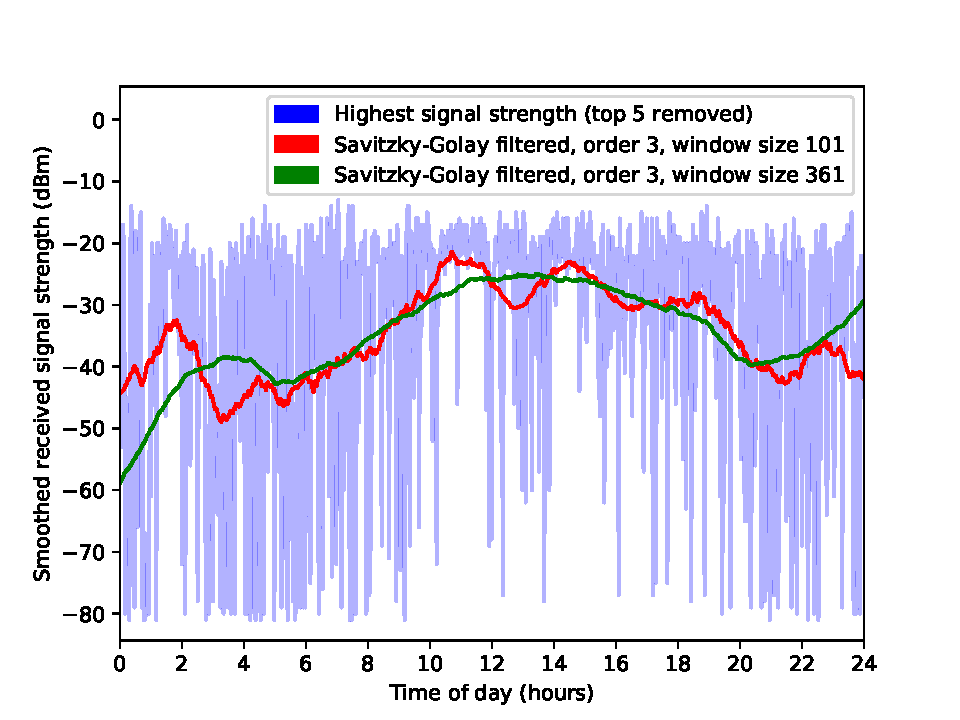
\includegraphics[width=\textwidth]{savitzky_1hour}
\caption{Savitzky-Golay smoothing, 1 additional hour of data point for each end.}
\label{savitzky_1}
\end{minipage}\
\end{figure}
\begin{figure}[htbp]
\begin{minipage}[t]{0.45\textwidth}
\centering
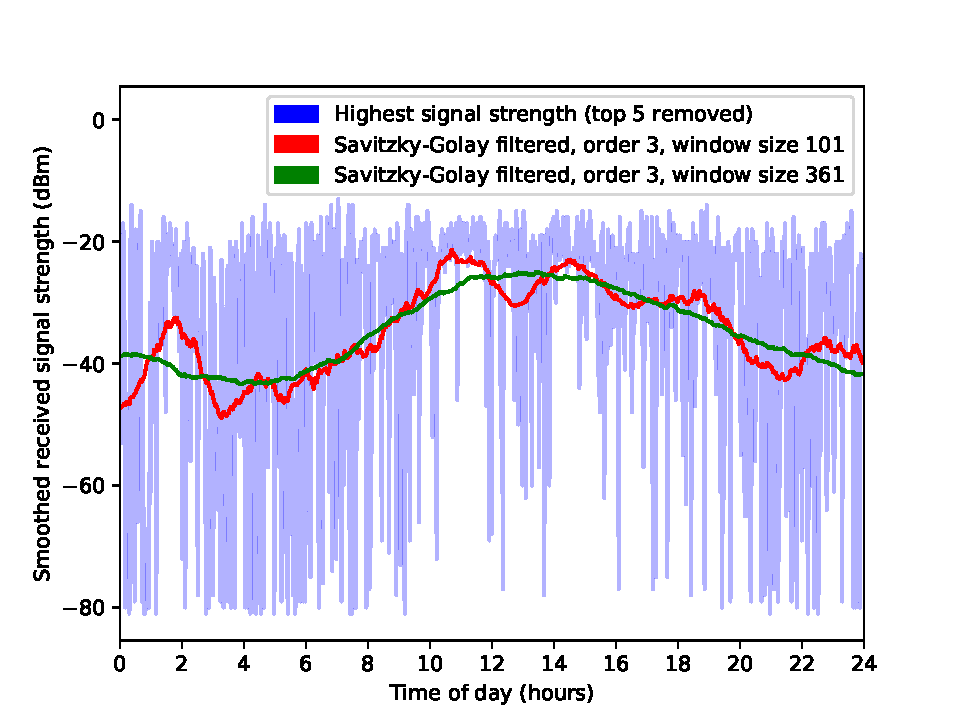
\includegraphics[width=\textwidth]{savitzky_4hours}
\caption{Savitzky-Golay smoothing, 4 additional hours of data points for each end.}
\label{savitzky_4}
\end{minipage}\

\end{figure}

We perform one scan per minute, alternating between 2.4GHz and 5.0GHz. As each scan takes at least 25 seconds to complete, we chose not to lower this interval any further. This generates around 860MB of raw data per node per day. Even when only considering the maximum signal strength per sample, we still need some way to condense this to a more digestible format. We experimented with some smoothing algorithms and had the best results with the Savitzky-Golay filter\footnote{\url{https://en.wikipedia.org/wiki/Savitzky\%E2\%80\%93Golay_filter}}. A detailed analysis of the filter was considered outside of the scope of this document, but we note that it is a digital filter intended for equally spaced data points that smooths data through convolution. We always used polynomials of degree 3. The only other parameter is the window size. The higher the window size, the smoother the final result. Figure \ref{savitzky_0} shows the resulting smoothings for 2 different window sizes. The smaller window size reveals some details such as the drop in activity between noon and 1PM (lunch time), while the larger window size is detailed enough to show that daytime is more active than nighttime. This filter performs well mainly for the center of the data set. The edges of the smoothing are clearly inaccurate, especially the sudden rise at the end of the day. This is a known issue with this filter. Luckily we usually also have the data of the preceding and following day. By starting the smoothing earlier and ending it later, we obtain a better smoothing. Figure \ref{savitzky_1} was generated using the data starting at 11PM the day before up to 1AM the day after. In figure \ref{savitzky_4} we increased this margin to 4 hours at each end. Whiel the 1 extra hour does little to improve the smoothing and even leads to a worse result in one case, the effect disappears completely with the 4 additional hours. We use this 4 hour buffer for all smoothings. Furthermore we decided to use the larger window size. The smoother graphs make it easier on the eye to compare multiple smoothings on one graph. Additionally effects such as the drop during lunchtime were often not seen with even tighter window sizes.\\
\newpage
\begin{wrapfigure}{r}{0.35\textwidth}
\centering
\captionsetup{justification=centering}
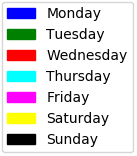
\includegraphics[width=0.25\textwidth]{legend.png}
\caption{Legend:\\ days of the week}
\label{legend}
\end{wrapfigure}
Using an adapted version of Simon W{\"u}nderlich's FFT$\_$eval code, Python's Matplotlib library, the mathematical formulas mentioned above and a Savitzky-Golay filter with window size 361 we graphically represent our data points per node. For one week (Monday 15 May - Sunday 21 May) we plot each day's smoothing, for easy comparison between the days. For the 2.4GHz band we perform this separately for the non-overlapping channels 1, 6 and 11. Each color in the plot represents a day of the week, using the legend in figure \ref{legend}. All other plots use the same legend, although days may be missing.



\subsection{Accuracy of the Measurements} \label{accuracy}

\begin{figure}[ht]
\begin{minipage}[t]{0.45\textwidth}
\centering
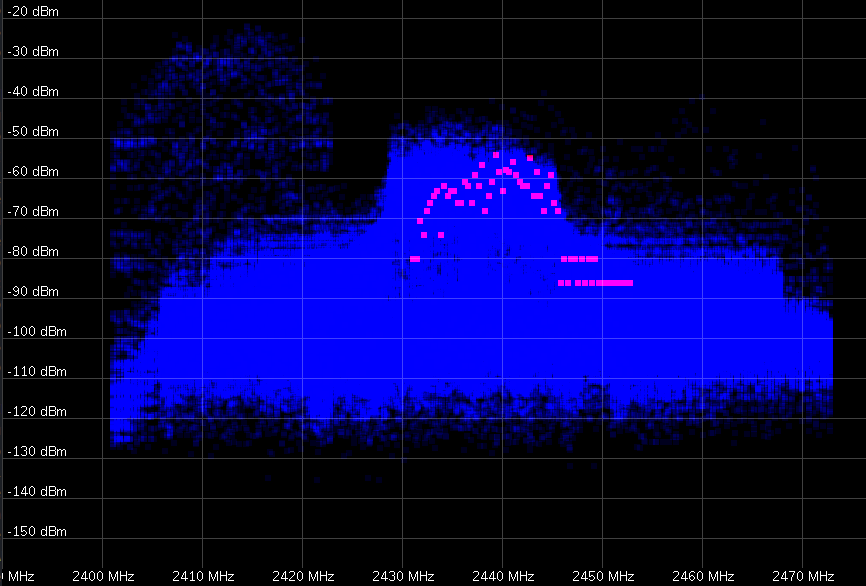
\includegraphics[width=\textwidth]{24check.png}
\caption{2.4GHz spectral scan with active nearby device at 2.437GHz.}
\label{fig_24}
\end{minipage}\hfill
\begin{minipage}[t]{0.45\textwidth}
\centering
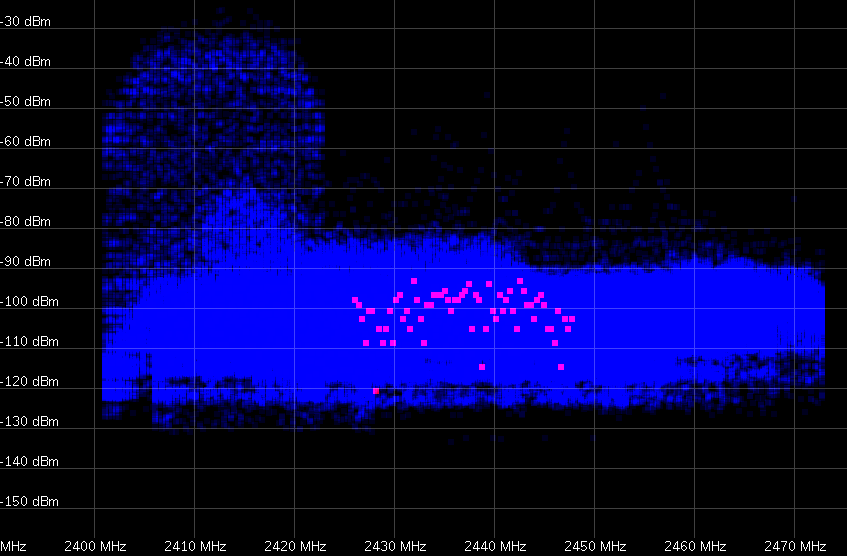
\includegraphics[width=\textwidth]{24check_nodata.png}
\caption{2.4GHz baseline spectral scan.}
\label{fig_24nodata}
\end{minipage}\
\end{figure}


\begin{figure}[ht]
\centering
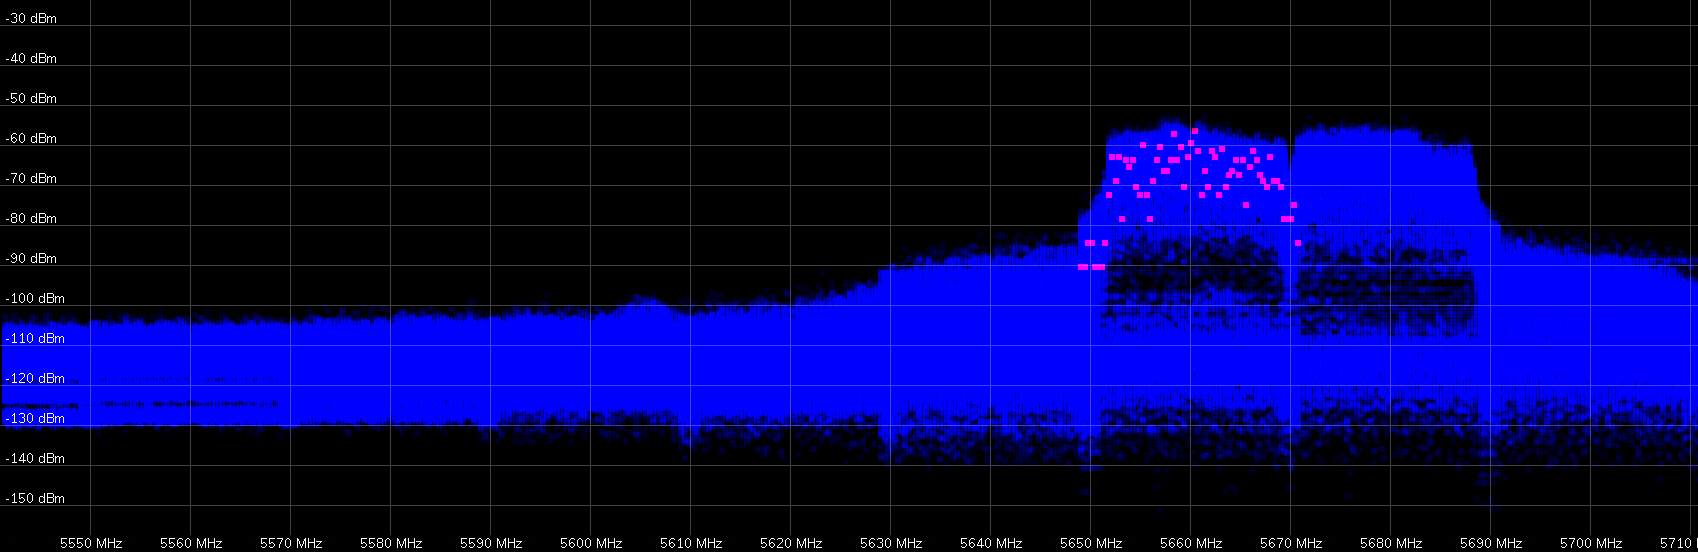
\includegraphics[width=0.75\textwidth]{50check.png}
% where an .eps filename suffix will be assumed under latex,
% and a .pdf suffix will be assumed for pdflatex; or what has been declared
% via \DeclareGraphicsExtensions.
\caption{5.0GHz spectral scan with active nearby device at 5.660GHz}
\label{fig_50}
\end{figure}

\begin{figure}[ht]
\centering
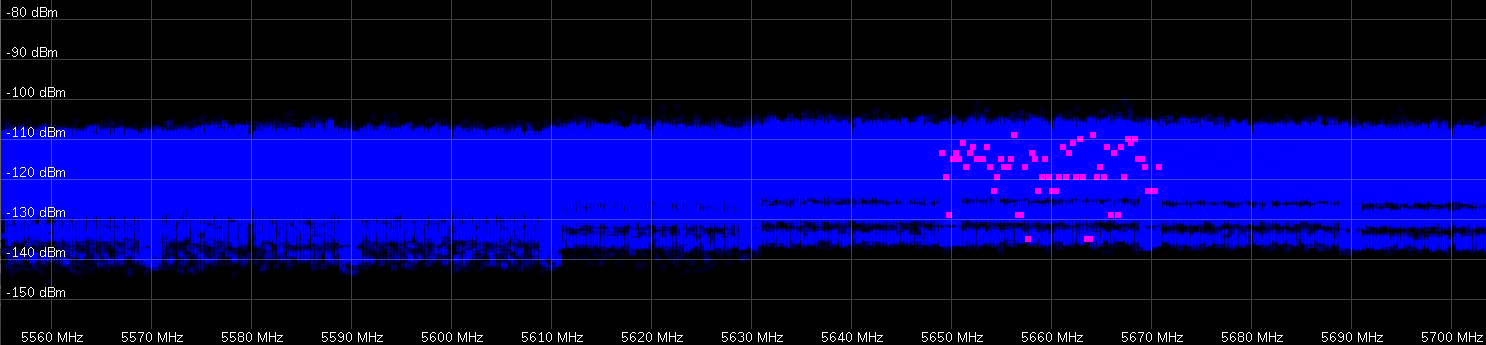
\includegraphics[width=0.75\textwidth]{50check_nodata.png}
% where an .eps filename suffix will be assumed under latex,
% and a .pdf suffix will be assumed for pdflatex; or what has been declared
% via \DeclareGraphicsExtensions.
\caption{5.0GHz baseline spectral scan.}
\label{fig_50nodata}
\end{figure}
We first confirm that the spectral scan does in fact accurately measure activity per channel. To test this, we perform a data transfer with a laptop positioned roughly 50cm from the node. We perform this on available 2.4GHz and 5.0GHz networks. The 2.4GHz network was using channel 6 (around 2.437GHz) and lead to the spectral scan in figure \ref{fig_24}. This scan shows a clear peak centered around channel 6 of around 20MHz wide. Figure \ref{fig_24nodata} shows a scan of the same node around the same time, but with our data transfer disabled. While the hazy peak around channel 1 is still there, the peak around channel 6 is not visible, indicating it was caused by our data transfer. Comparing the two, we see that our data transfer caused an increase in received signal strength of around 40dBm.\\ Our 5.0GHz test was using an access point centered around channel 132 (5.66GHz) and lead to figure \ref{fig_50}. Compared to the flat \ref{fig_50nodata} captured with the data transfer disabled, the peak is again very clear. Received signal strength is increased by up to 50dBm in this case. The scan is detailed enough to indicate that the access point was using a 40MHz wide channel: data is being transferred both in channel 132 (5.66GHz) and channel 136 (5.68Ghz). These two tests clearly show that this method is accurate enough for our goals.



\section{Results}
In this section we present the results of our experiment. Due to (presumed) hardware failure, some measurements failed. As a result we had to limit and/or shift the timeframe of the presented measurements for some nodes. This is indicated below.
\subsection{Evolution throughout the day}

\subsection{Recurring patterns between days} 
On the different nodes we had varying degrees of success in finding recurring patterns. In the 2.4 GHz band, two nodes that clearly showed repeating patterns across several days were node 8 at the Museum Plantin-Moretus and node 12 at the University of Antwerp, Middelheim campus. Both of these nodes detected patterns, with node 8 detecting a large increase in spectrum usage in the afternoon and node 12 detecting an increase during the daytime on weekdays. There were no peaks during the weekend. Node 8 was one of the nodes with failure, so we had to limit its timeframe.

\begin{figure}[!h]
\begin{minipage}{0.47\textwidth}
    \centering
	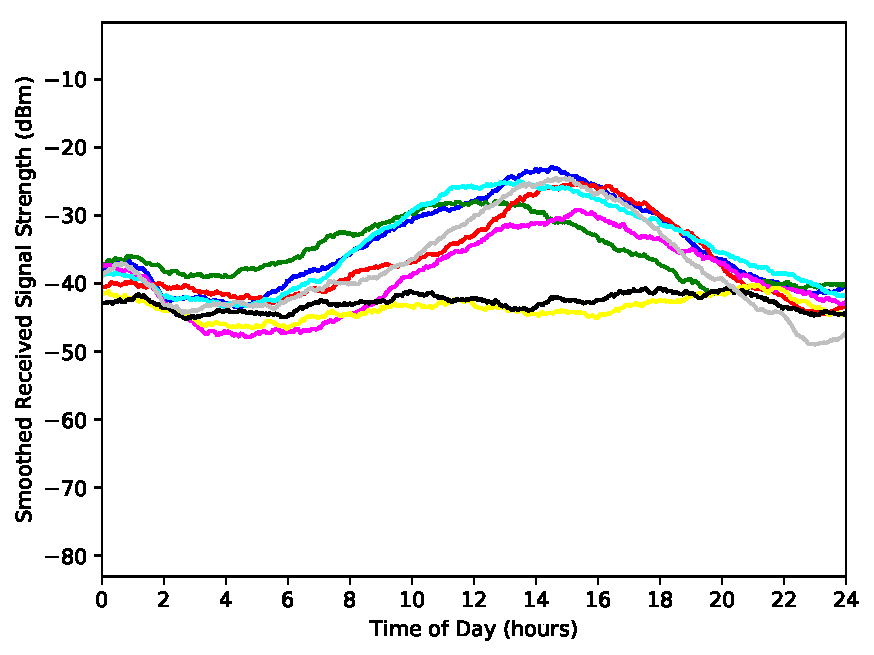
\includegraphics[width=\textwidth]{images/2_4_GHz/cot-node12-student_2017-05-22_chan1_image}
    \caption{Node 12, ch. 1, 15/05 - 22/05} \label{node12-1}
\end{minipage}\hfill
\begin{minipage}{0.47\textwidth}
    \centering
	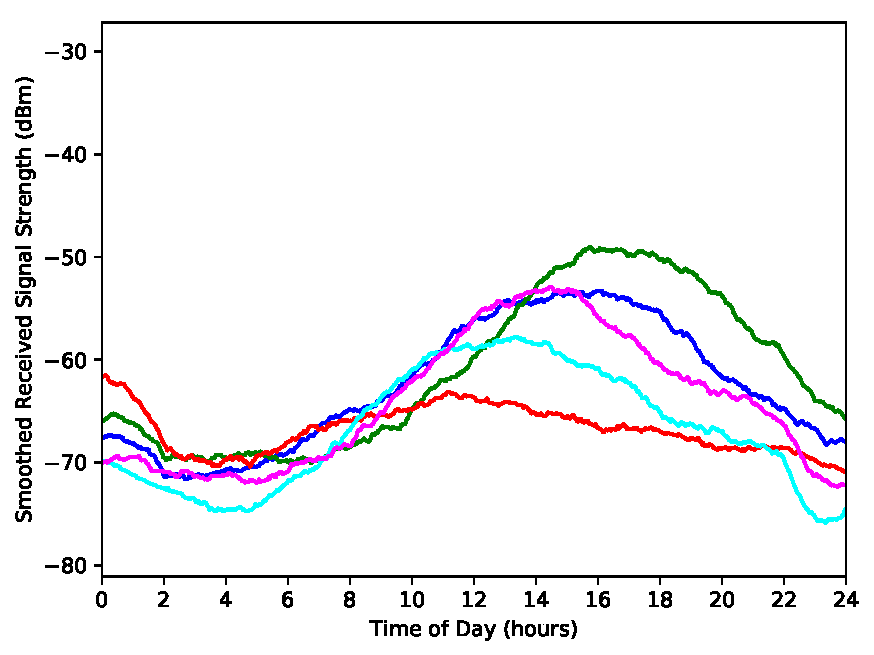
\includegraphics[width=\textwidth]{images/2_4_GHz/cot-node8-student_2017-05-16_chan1_image}
    \caption{Node 8, ch. 1, 12/05 - 16/05} \label{node8-1}
\end{minipage}\hfill
\end{figure}
\begin{figure}[!h]
\begin{minipage}{0.47\textwidth}
    \centering
	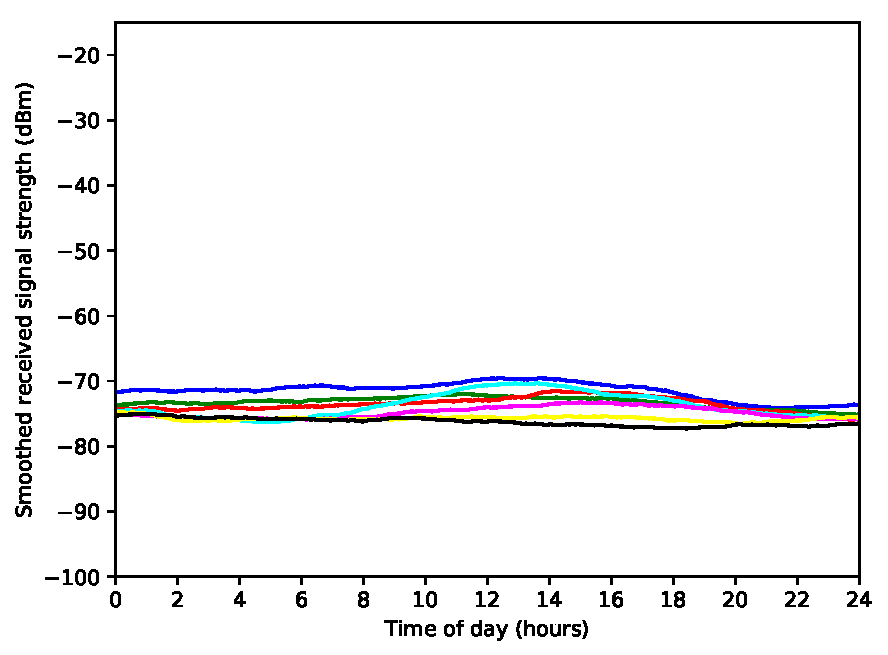
\includegraphics[width=\textwidth]{images/2_4_GHz/cot-node12-student_2017-05-22_chan6_image}
    \caption{Node 12, ch. 6, 15/05 - 22/05} \label{node12-6}
\end{minipage}\hfill
\begin{minipage}{0.47\textwidth}
    \centering
	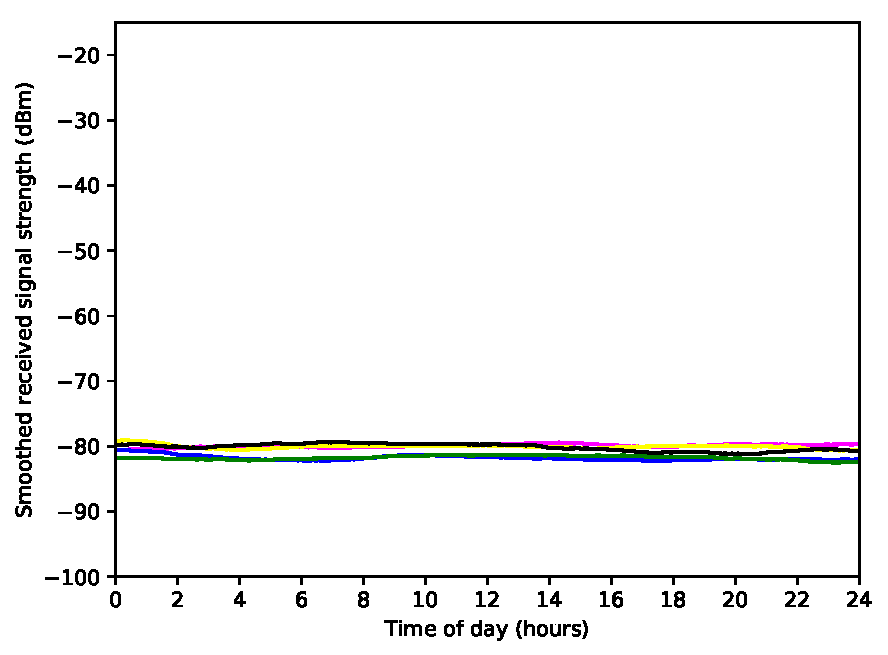
\includegraphics[width=\textwidth]{images/2_4_GHz/cot-node8-student_2017-05-16_chan6_image}
    \caption{Node 8, ch. 6, 12/05 - 16/05} \label{node8-6}
\end{minipage}\hfill
\end{figure}
\begin{figure}[!h]
\begin{minipage}{0.47\textwidth}
    \centering
	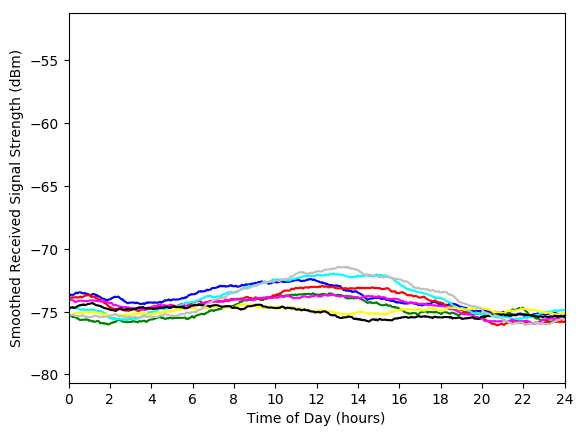
\includegraphics[width=\textwidth]{images/2_4_GHz/cot-node12-student_2017-05-22_chan11_image}
    \caption{Node 12, ch. 11, 15/05 - 22/05} \label{node12-11}
\end{minipage}\hfill
\begin{minipage}{0.47\textwidth}
    \centering
	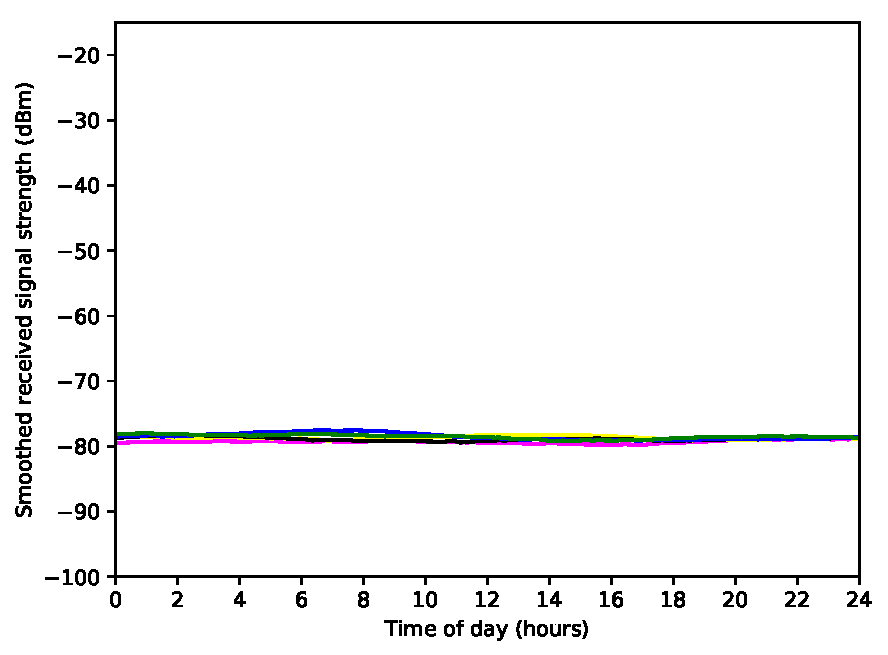
\includegraphics[width=\textwidth]{images/2_4_GHz/cot-node8-student_2017-05-16_chan11_image}
    \caption{Node 8, ch. 11, 12/05 - 16/05} \label{node8-11}
\end{minipage}\hfill
\end{figure}

The most noticeable peak for node 12 is on channel 1, with the received signal strength during the daytime being up to 20dBm higher than during the night time. During the weekend (black and yellow) there is no peak whatsoever. This indicates the traffic is most likely caused by Wi-Fi usage at the university, which is closed during the weekend. For the other channels there a noticeable peak during the daytime for some but not all weekdays. The weekend is still the quietest time of the week. Node 8 also shows a peak during the afternoon for channel 1, except on Sunday. Surprisingly the museum is open on Sunday, but closed on Monday. Of the days with a peak, Monday's peak is the lowest. This seems to indicate that while visitors at the museum have some effect on the overall signal strength, the peak has another source, possibly an office nearby. \\ \\
We found no such peaks for any other nodes: spectrum usage was stable throughout the day. In the following section we investigate how active the different channels are.


\subsection{Channel Activity}

\begin{figure}[!h]
\begin{minipage}{0.47\textwidth}
    \centering
	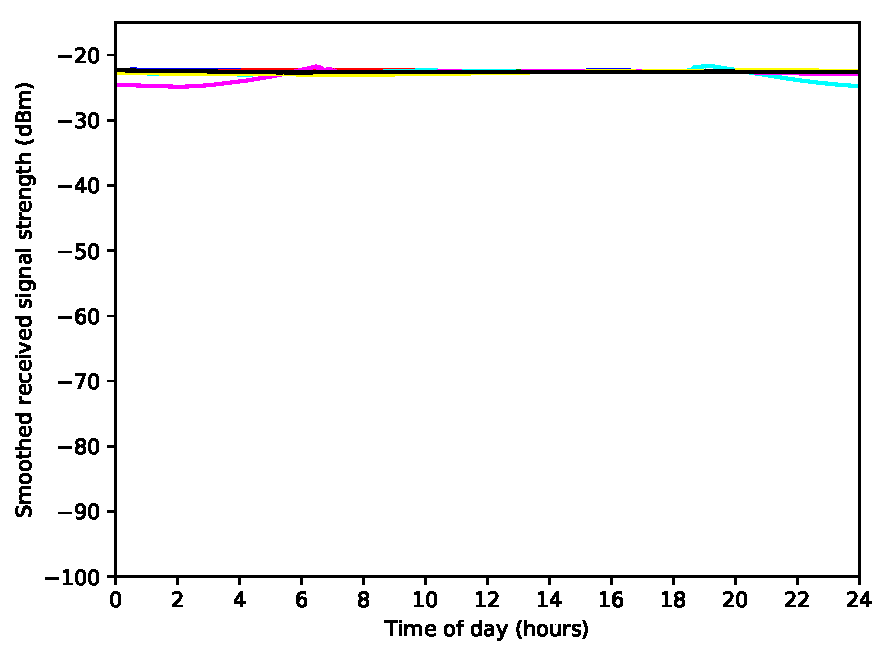
\includegraphics[width=\textwidth]{images/2_4_GHz/cot-node3-student_2017-05-21_chan1_image}
    \caption{Node 3, ch. 1, 15/05 - 22/05} \label{node3-1}
\end{minipage}\hfill
\begin{minipage}{0.47\textwidth}
    \centering
	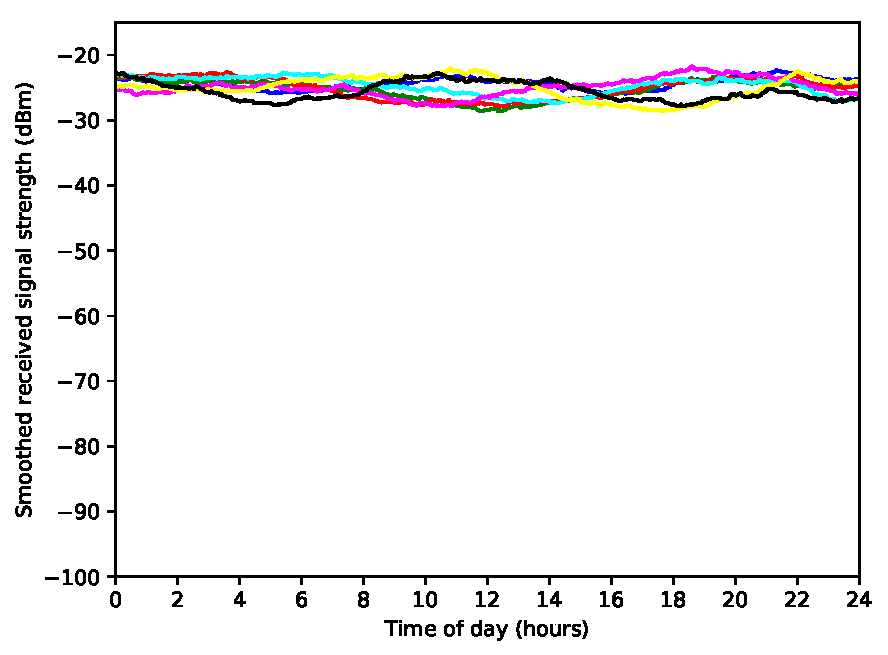
\includegraphics[width=\textwidth]{images/2_4_GHz/cot-node9-student_2017-05-21_chan1_image}
    \caption{Node 9, ch. 1, 15/05 - 22/05} \label{node9-1}

\end{minipage}\hfill
\end{figure}
\begin{figure}[!h]
\begin{minipage}{0.47\textwidth}
    \centering
	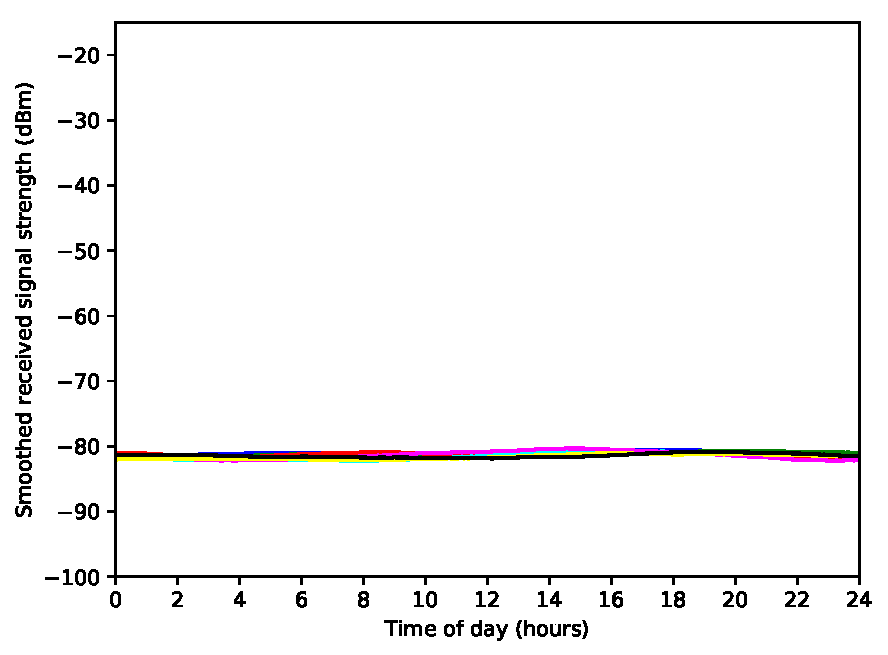
\includegraphics[width=\textwidth]{images/2_4_GHz/cot-node3-student_2017-05-21_chan6_image}
    \caption{Node 3, ch. 6, 15/05 - 22/05} \label{node3-6}
\end{minipage}\hfill
\begin{minipage}{0.47\textwidth}
    \centering
	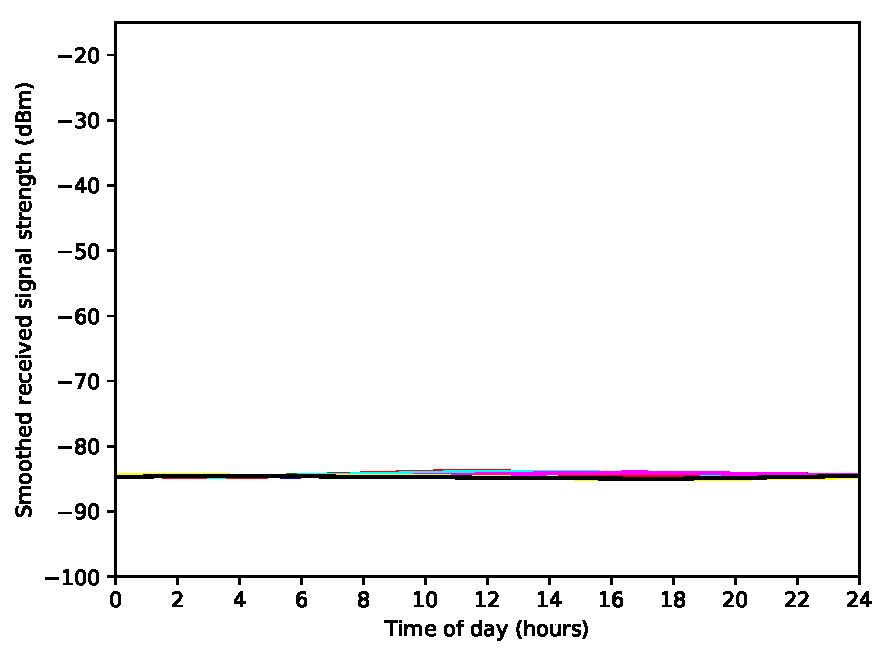
\includegraphics[width=\textwidth]{images/2_4_GHz/cot-node9-student_2017-05-21_chan6_image}
    \caption{Node 9, ch. 6, 15/05 - 22/05} \label{node9-6}
\end{minipage}\hfill
\end{figure}

\begin{figure}[!h]
\begin{minipage}{0.47\textwidth}
    \centering
	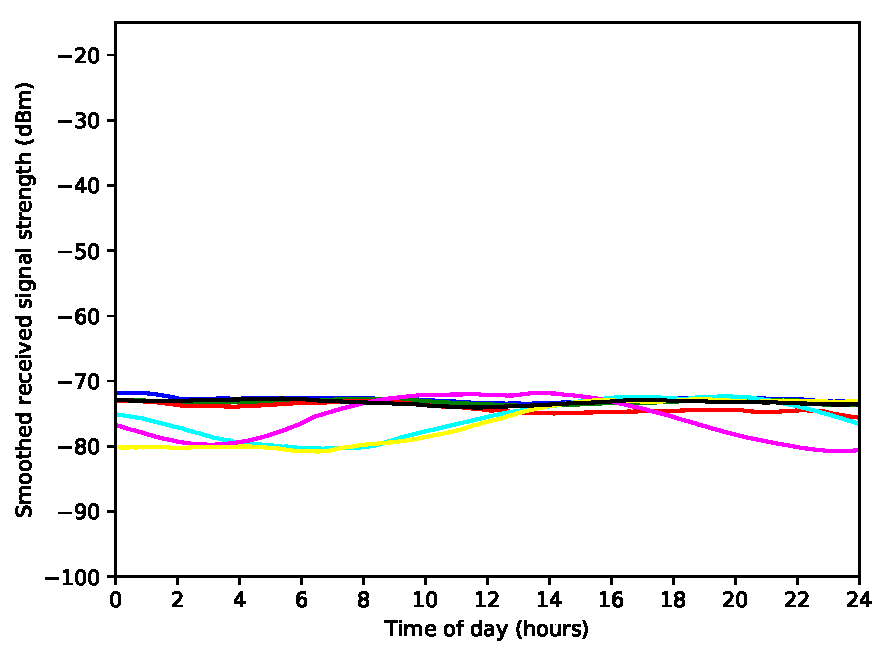
\includegraphics[width=\textwidth]{images/2_4_GHz/cot-node3-student_2017-05-21_chan11_image}
    \caption{Node 3, ch. 11, 15/05 - 22/05} \label{node3-11}
\end{minipage}\hfill
\begin{minipage}{0.47\textwidth}
    \centering
	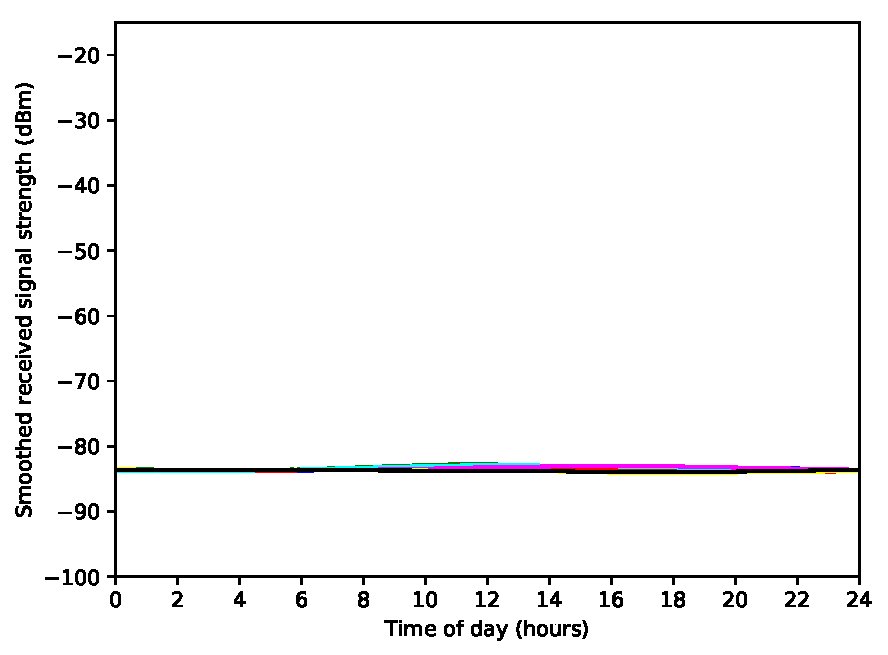
\includegraphics[width=\textwidth]{images/2_4_GHz/cot-node9-student_2017-05-21_chan11_image}
    \caption{Node 9, ch. 11, 15/05 - 22/05} \label{node9-11}
\end{minipage}\hfill
\end{figure}



As shown in figures \ref{node3-1} to \ref{node9-11}, channel 1 is usually the busist channel in the 2.4 GHz band, with channels 6 and 11 trailing far behind. Node 3 and 9, shown in those figures, measure a very busy medium around channel 1. However channels 6 and 11 are not particulary busy compared to the traffic seen on the other nodes, as we can see from these graphs:\\

\newpage
All nodes covered so far were indoors node. We had access to one outdoors node, node 1, on which we also performed the experiment. On the indoors nodes we noticed that channel 6 and 11 were never any busier than channel 1. This is also true for node1: while activity is fairly constant throughout all tested days, channel 1 is again the busiest. Note that we again do not have a full week's data for this note. Note the remarkable difference between weekdays and the weekend here. For channel 11, the weekend is more quiet, however for channel 6 the weekend is the busiest period.
\begin{figure}[!h]
\begin{minipage}{0.47\textwidth}
    \centering
	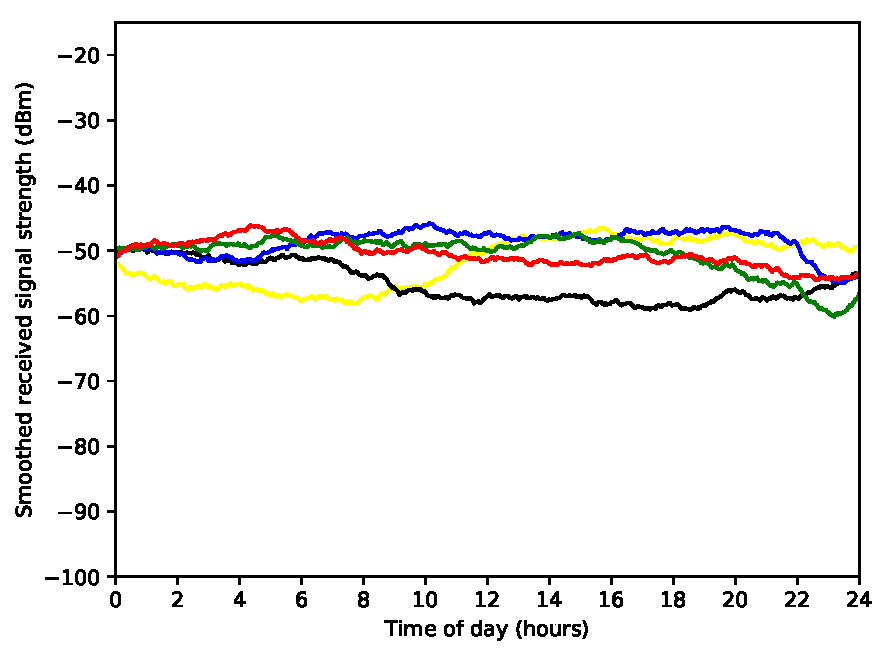
\includegraphics[width=\textwidth]{images/2_4_GHz/node1_2017-05-17_chan1_image}
    \caption{Node 1, ch. 1, 13/05 - 17/05} \label{node1-1}
\end{minipage}\hfill
\begin{minipage}{0.47\textwidth}
    \centering
	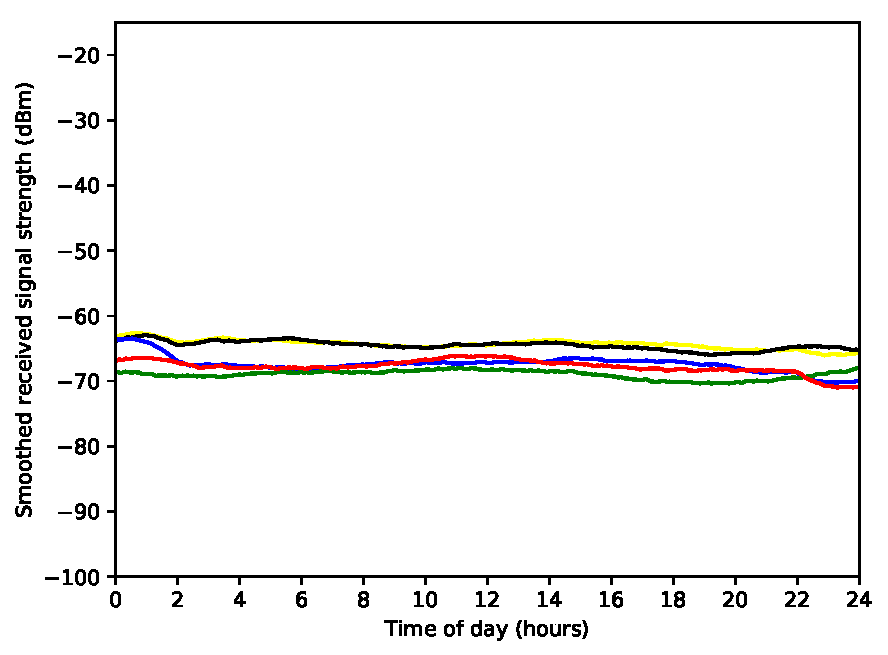
\includegraphics[width=\textwidth]{images/2_4_GHz/node1_2017-05-17_chan6_image}
    \caption{Node 1, ch. 6, 13/05 - 17/05} \label{node1-6}
\end{minipage}\hfill
\end{figure}
\begin{figure}[h!]
\begin{minipage}{0.47\textwidth}
    \centering
	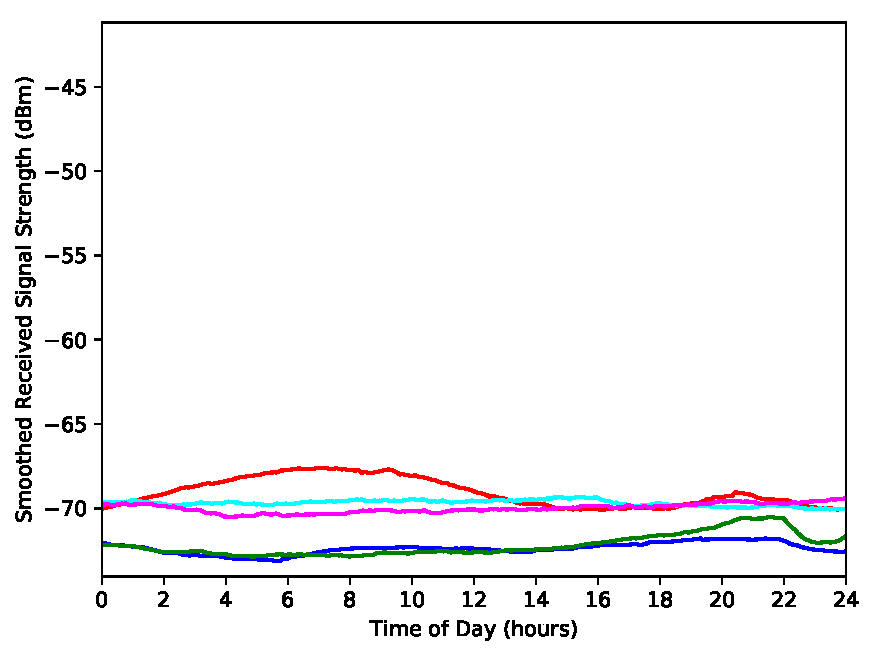
\includegraphics[width=\textwidth]{images/2_4_GHz/node1_2017-05-17_chan11_image}
    \caption{Node 1, ch. 11, 13/05 - 17/05} \label{node1-11}
\end{minipage}\hfill
\end{figure}
%\begin{figure}[h!]
%    \centering
%    \textbf{node1, channel 11, 13/05 - 17/05}\par\medskip
%	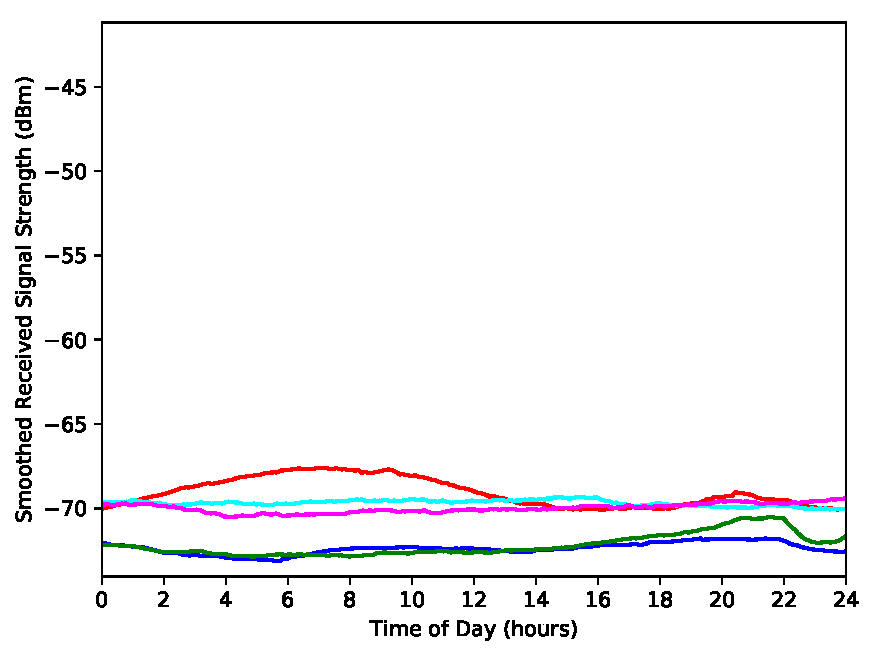
\includegraphics[scale=0.5]{images/2_4_GHz/node1_2017-05-17_chan11_image}
%\end{figure}
\subsection{2.4 GHz vs 5 GHz}
niks van de 5ghz bevat iets zinnigs (op node3 / chan36 na) - nodes te ver weg ?
>> still running the graph generator for 5GHz to compare lol
\subsection{Validation}
While there is no official confirmation from the chip manufacturer that our interpretation of the spectral scan data is correct, we are confident that our interpretation gives at least a solid estimation of spectrum activity. First of all the experiment in section \ref{accuracy} shows that when we add a source of RF activity near the node, this is clearly seen in the spectral scan at exactly the right frequency. \\
Furthermore we discovered daily patterns where we expected them. The Middelheim offices are busy during the daytime on weekdays but fairly silent during the weekends and nights. While not shown in the plots above, holidays were just as quiet as weekends.

\section{Conclusions}
In this report we presented our findings on activity in the RF spectrum in the 2.4GHz and 5.0GHz bands in the city of Antwerp. One clear theme in our results is that the 5.0GHz is overall quieter than the 2.4GHz band. This is not surprising. The 5.0GHz band is a lot wider than the 2.4GHz band, and its signals do not carry as far. Furthermore, assuming that a lot of interference originated from Wi-Fi routers, one factor could be that many active routers and other devices do not yet support 5.0GHz. In addition, technologies such as Bluetooth, which could also be creating signals, only work on 2.4GHz.\\ \\
In some environments we notice a daily pattern where the signal strength is about 20dBm higher during the day compared to the night. As this was mainly observed on nodes in office spaces, this effect disappeared during the weekend. Other nodes show absolutely no difference between daytime and nighttime. Often this is when the spectrum is just very quiet. One interesting observation is that channels 6 and 11 were never busier than channel 1. 
\bibliographystyle{IEEEtran}
\bibliography{IEEEabrv,./bibliography}




% that's all folks
\end{document}
